\documentclass[11pt]{article}
\usepackage[margin=1in]{geometry}
\usepackage{amsmath,amssymb}
\usepackage{booktabs}
\usepackage{graphicx}
\usepackage{hyperref}
\usepackage{caption}
\usepackage{float}
\hypersetup{colorlinks=true,linkcolor=blue,citecolor=blue,urlcolor=blue}

\title{Redshift from delay growth on a closed integer lattice:\\
the law, its kinematic correspondence to a scale factor, and the supernova test}
\author{Alon Gonen\\
\small Independent researcher\\
\small \texttt{alon@defounder.ai} \quad ORCID 0009-0008-2701-4599}
\date{September 2026}

\begin{document}
\maketitle

\begin{abstract}
On a closed lattice whose computation load grows with age, and whose rule
delays the transport of light but not local cycles, a signal that crosses $D$
links arrives stretched: rays emitted one hop apart, $k_e$ ticks, reach an
eye $k_o$ ticks apart on the eye's own clock, so $1 + z = k_o / k_e$, the
ratio of the hop time at reception to the hop time at emission, and
durations stretch by the same ratio. We measure this on the Universe24
simulator (bounded integers, one Link per tick) with a train of twelve
single-quantum rays crossing closed rows of 16 to 96 Nodes to an absorbing
eye that counts its own cycles: the per-run ratio holds within a tick per
gap, the eye's clock keeps the bare rate with rays waiting at it, the
stretch grows with the distance as $1 + z = e^{\alpha D}$ with $\alpha$ read
off the hop schedule, and $\alpha$ scales with the emission. One source
emitting twelve rays at a fixed interval of its own clock, all crossing the
same 47 links, gives the same law: $z = 1.07$, with the gaps at the eye over
the interval at the source, $2.07$, against the ray-by-ray $k_o/k_e$ of
$2.03$. The wave sector is measured too: with the default rule, a phase
that advances per link, the frequency of a phased-ray train redshifts with
the rate, $\nu_o/\nu_e = 0.58$ at $z = 0.77$ against $1/(1+z) = 0.56$; with
the phase advancing per waiting interval as well, only the frequency's
excess over the advance rate redshifts. A train of moving bodies, the first
choice of light, is not usable: a Node starts no new cycle until its delayed
departure has arrived, so bodies stall the clocks of the Nodes they wait at.
We then show a kinematic correspondence: with $D = \int dt/k$ the hop time
$k(t)$ plays the part of $a(t)$ in a Friedmann universe for the Hubble
diagram and the time dilation, so those two tests are reproduced by a
static lattice with the matching load history, and the question of dark
energy becomes the question of what makes the load grow. The luminosity
distance needs two further readings that are assumed, not measured here: a
$1/D^2$ dilution, and that a quantum's energy follows its frequency
(reading B). Against the Pantheon+ supernova sample (1580 Hubble-flow
objects, one free offset, full statistical-plus-systematic covariance) the
two histories the model supplies on its own, constant emission ($k \propto
t$, coasting) and emission growing with age ($k \propto t^2$, $q_0 = -1/2$),
are disfavoured by $\Delta\chi^2 = 106$ and $64$ against flat
$\Lambda$CDM, while a power law $k \propto t^{1.4}$ fits within
$\Delta\chi^2 = 9$; the reading in which only the arrival rate is
redshifted fails at every exponent. The Tolman surface-brightness exponent
separates the lattice from expansion, $(1+z)^{-2}$ against $(1+z)^{-4}$; the
measured exponent lies above the lattice's, so the model is in tension
there now, and we say what would relieve it. Nothing here removes dark
energy: the acceleration is relabelled as a load history that the model
does not yet derive.
\end{abstract}

\section{Introduction}

A redshift without recession has been proposed many times, from tired light
\cite{zwicky1929} to varying-constant cosmologies, and has been tested
against the same three observations each time: the supernova Hubble diagram
\cite{riess1998,perlmutter1999,scolnic2022,brout2022}, the time dilation of
supernova light curves \cite{blondin2008}, and the Tolman surface-brightness
relation \cite{lubin2001}. Classic tired light fails the second and third.
This paper reports a mechanism of a different kind, measured on a bounded
integer lattice simulator, and puts it to the same three tests without
softening them.

The mechanism is not a loss of energy along the path. It is a growth of the
time a hop takes, everywhere and with age, while local cycles keep their bare
time: a universal slowing of transport read by clocks that do not slow. Such
a rule is a configured hypothesis of the Universe24 simulator (a computation
field whose load prices departures, postulate on computation cost), and the
first paper on that simulator \cite{paper1} kept its cosmological
consequences on a hypotheses page. Here they are measured, mapped onto the
standard language, and tested against data.

Three things are established. First, the law on the lattice: $1 + z = k_o /
k_e$ within a tick per gap, for a train and for a single source, with time
dilation by the same factor, and its continuum form for each load history.
Second, a kinematic correspondence: the hop time is a scale factor for the
Hubble diagram and the time dilation, so the lattice reproduces those two
tests of any Friedmann model with the matching load history and cannot be
told from expansion by them alone; the correspondence is kinematic because
nothing dynamical (no Friedmann equation, no equation of state) is derived.
Third, the data: the load histories the model supplies by itself do not fit
the supernova diagram, a fitted power law does, and the surface-brightness
exponent is where the lattice and expansion part, with the measured value on
expansion's side. The conclusion is negative for the strong claim
(no dark energy) and positive for a narrower one (a lattice mechanism that
carries the whole Hubble diagram in one function, with a stated test).

\section{The lattice and the rule}\label{sec:rule}

Universe24 is a lattice of Nodes joined by six Links; every quantity is a
bounded integer; a packet crosses one Link per tick; each Node runs local
cycles priced in configured operation costs. A configured conserved field
may be named the computation field: its local load $C$ adds to the cost of
a cycle at the Node, and a cycle whose cost exceeds the normal budget $B$
takes $k = \lceil C / B \rceil$ intervals. Two opt-in rules of the simulator
carry the whole physics of this paper. With directional delay
(\texttt{delay\_direction: along}) the load prices only the departures of
moving records, and local updates commit after the bare cycle time: a held
record's clock does not slow. With ray delay (\texttt{ray\_delay}) a ray of
a straight-ray field resident at a Node waits $\lceil C/B \rceil - 1$ extra
field cycles before it is forwarded, so a hop takes $k$ ticks; a waiting ray
stalls no record. Transport slows with the load, clocks do not.

The configuration is a closed row of $L$ Nodes (periodic in $x$, one Node
across). Every Node holds a mass body that emits a constant amount $E$ of
the computation field per cycle, so the field's total grows linearly with
age and, by symmetry, the load at every Node grows alike: the row is a
closed universe filling uniformly with field, and the hop time rises by one
every $B/\lambda$ ticks for a load growing by $\lambda$ per tick. Light is a
train of twelve single-quantum rays: twelve lamps at $x = 0, \dots, 11$ each
emit one ray heading $+x$ at tick 1, so the rays are one link apart and, at
any Node they pass, one hop apart in time. Each ray carries its lamp's label,
so rays never merge. In the single-source configuration the twelve lamps
sit on one Node at $x = 0$ and each emits once, the $i$-th when that Node's
own clock reads $3 i k_e$ ticks (three launch hops apart, because the rule
holds one wait register per Node and rays closer in time than the hop time
would leave together), so every ray crosses the same $L - 1$ links and the
interval at the source is set by the source's clock rather than by the
lamps' spacing. An eye at $x = L-1$ absorbs every ray that reaches it
(twelve quanta conserved into its inventory) and counts its own cycles: its
clock. The rays leave one hop apart, $k_e$ ticks, and are absorbed $k_o$
ticks apart, so the stretch the eye reads is (with the single source, the gap at the
eye over the interval at the source, and $k_o/k_e$ read ray by ray)
\begin{equation}
1 + z = \frac{k_o}{k_e}, \qquad \text{and, for the whole train,}\qquad
\frac{\text{duration at reception}}{\text{duration at emission}} = 1 + z,
\label{eq:law}
\end{equation}
both of which the lattice states as integers. Equation \eqref{eq:law} follows from the rule by construction, since every hop takes the hop time in force; what is not given by construction, and what the runs establish, is that an eye reads it on its own clock, that the wave's frequency follows it, and how the distance enters. The distance enters through the travel time: $D$ hops each taking $k(t)$ ticks give
\begin{equation}
D = \int_{t_e}^{t_o} \frac{dt}{k(t)},
\label{eq:distance}
\end{equation}
so for $k$ linear in age, $k = k_e + \lambda t/B$, $D = (1/\alpha)\ln(1+z)$
with $\alpha = \lambda/B$ per hop, the rate at which the hop time rises, an
exponential law; for $k \propto t^n$, $D \propto (1+z)^{(n-1)/n} - 1$.

\paragraph{Why rays.} The first version of this experiment used a train of
moving bodies for light. Under directional delay a body's departure waits
for the load, and a Node starts no new cycle until its slowest departure has
arrived, so the clocks of the Nodes a train waits at are stalled while it
waits: on a 24-row with constant emission the emitters completed 320 to 436
cycles in 700 ticks with the train present and 700 without it, and an
observer that hosts the bodies' departures reads no stretch on its own
clock. Rays wait without stalling anyone, and the eye's cycle count equals
the tick count in every run below. This is a measured property of the rule,
not a choice of convenience, and it is reported because a redshift that only
the global tick can see is not an observation.

\section{Measurements}\label{sec:measure}

\begin{table}[H]\centering\footnotesize\setlength{\tabcolsep}{3pt}
\begin{tabular}{p{2.9cm}p{2.9cm}rrrrrrr}
\toprule
Run & row, $E$, $B$, baseline & $D$ & $k_e$ & $z$ & $k_o/k_e$ & duration & $\alpha_{\rm meas}$ & $\alpha_{\rm sched}$\\
\midrule
row 16 & 16, 16, 1000, 7000 & 9.5 & 8 & 0.068 & 1.062 & 1.068 & 0.0069 & 0.0116\\
row 24 & 24, 16, 1000, 7000 & 17.5 & 8 & 0.216 & 1.208 & 1.216 & 0.0112 & 0.0145\\
row 32 & 32, 16, 1000, 7000 & 25.5 & 8 & 0.386 & 1.375 & 1.386 & 0.0128 & 0.0155\\
row 48 & 48, 16, 1000, 7000 & 41.5 & 8 & 0.773 & 1.760 & 1.773 & 0.0138 & 0.0158\\
row 64 & 64, 16, 1000, 7000 & 57.5 & 8 & 1.296 & 2.281 & 2.296 & 0.0145 & 0.0158\\
row 96 & 96, 16, 1000, 7000 & 89.5 & 8 & 2.807 & 3.781 & 3.807 & 0.0149 & 0.0159\\
control, no emission & 48, 0, 1000, 7000 & 41.5 & 7 & 0.000 & 1.000 & 1.000 & n/a & n/a\\
half the emission & 48, 8, 1000, 7000 & 41.5 & 8 & 0.284 & 1.281 & 1.284 & 0.0060 & 0.0073\\
double the emission & 48, 32, 1000, 7000 & 41.5 & 8 & 2.329 & 3.281 & 3.329 & 0.0290 & 0.0318\\
launch at k = 1 & 48, 16, 1000, 900 & 41.5 & 1 & 1.818 & 2.750 & 2.818 & 0.0250 & 0.0154\\
launch at k = 4 & 48, 16, 1000, 3000 & 41.5 & 4 & 0.659 & 1.646 & 1.659 & 0.0122 & 0.0150\\
launch at k = 16 & 48, 16, 1000, 15000 & 41.5 & 16 & 0.830 & 1.818 & 1.829 & 0.0146 & 0.0159\\
single source & 48, 16, 1000, 7000 & 47.0 & 8 & 1.068 & 2.032 & 2.068 & 0.0155 & 0.0160\\
single source, no emission & 48, 0, 1000, 7000 & 47.0 & 7 & 0.000 & 1.000 & 1.000 & n/a & n/a\\
\bottomrule
\end{tabular}
\caption{The closed-row runs. $D$ is the mean distance from the twelve lamps to the eye ($L - 1$ for the single source); $z$ is the mean gap between consecutive absorptions on the eye's clock divided by the interval at the source ($k_e$ for the train, $3 k_e = 24$ ticks for the single source), minus one; $k_o/k_e$ is the mean hop time in force while the train is absorbed over the hop time at launch (ray by ray for the single source, whose launch hop rises during the emission); duration is the train's span at the eye over its span at launch; $\alpha_{\rm meas} = \ln(1+z)/D$; $\alpha_{\rm sched}$ is the rate at which the hop time rose during the run, read off every ray's hops. In every run the eye's clock equals the tick count, the field's total grows linearly, and the twelve quanta are conserved.}
\label{tab:runs}
\end{table}

\paragraph{The law.} In every run the twelve rays are absorbed, the twelve quanta are conserved, the
field's total grows linearly with age, and the eye's cycle count equals the tick
count at every absorption, so the gaps on the eye's clock are the gaps in
ticks. The control without emission gives gaps of $k_e$ and $z = 0$ (its launch hop is 7 rather than 8, since no emission lifts the load past seven budgets on the first tick).
With emission the gaps grow along the train (13, 13, 14, \dots, 15 on the
48-row), because the hop time rises while the train is absorbed; their mean
over $k_e$ minus one is $z$, the train's span at the eye over its span at
launch is $1 + z$ in every run (the duration column, the same integers
read twice), and the mean hop time of the rays' last hops over $k_e$ agrees
with $1 + z$ within one tick per gap ($3.78$ against $3.81$ on the 96-row):
the law holds to the resolution of the integers, which is what ``holds''
means on this lattice. Every hop's duration
equals $\lceil (b + \lambda t)/B \rceil$ at the tick it began, with $\lambda$
the emission per Node per tick: the law is the ceiling of the load over the
budget, and nothing else.

\paragraph{One source.} The train reads the law off twelve lamps at
twelve distances launched at one tick. The single-source run removes both
conveniences: one Node emits every 24 ticks of its own clock (three launch
hops at $k_e = 8$), every ray crosses the same 47 links, and the emission
spans 264 ticks during which the launch hop rises from 8 to 12. The eye's
gaps are 47 to 52 ticks, mean $49.6$, against 24 at the source: $z =
1.068$, the duration ratio $2.068$, against the ray-by-ray $k_o/k_e$ of
$2.032$, a difference of one tick in a gap of fifty. The continuum law
gives $\ln(1+z) = 0.0160 \times 47 = 0.750$, $z = 1.12$, and with the
train's launch offset of $0.065$ (a launch at $k_e = 8$ with the load at
$7.02$ budgets) $z = 0.98$; the measured $1.07$ lies between, within a tick
per gap of either, as it should for launches spread over 264 ticks across
five steps of the ceiling, whose offsets average smaller than the train's
single one. Without emission the same source gives gaps of 24 and $z = 0$. The stretch is therefore not an artefact of the train's
geometry: a source with a clock, an interval and a distance is redshifted
by the interval at the source over the interval at the eye, as the law
states.

\paragraph{Distance and size.} The six rows at one emission put the eye at $D = 9.5$ to $89.5$ links from the
lamps: $z = 0.068, 0.216, 0.386, 0.773, 1.296, 2.807$. The stretch depends on
the distance and on nothing else about the row; $\ln(1+z)/D$ rises from
$0.0069$ at $9.5$ links to $0.0149$ at $89.5$ and approaches the slope of the
hop schedule, $0.0158$ per link ($\lambda/B = 0.016$). The shortfall at short
distance is the launch offset of the ceiling: the hop time at launch is
$k_e = 8$ while the load then stands at $7.02$ budgets, so the continuum
integral \eqref{eq:distance} runs from $7.5$ rather than $8$ and
$\ln(1+z) = \alpha D - \ln(k_e/(u_e + \tfrac12)) = \alpha D - 0.065$, which
gives $z = 0.09, 0.81$ and $2.86$ at $9.5$, $41.5$ and $89.5$ links against
the measured $0.07, 0.77$ and $2.81$.

\paragraph{Emission.} At $D = 41.5$ the stretch follows the emission: $z = 0.284$ at half the
emission and $0.773$ at the reference, with hop-schedule slopes $0.0073$ and
$0.0158$ per link (the ratio $0.46$ is the ceiling's rounding at a slower
rise); at double the emission $z = 2.329$, with slope $0.0318$ per link, twice the reference's $0.0158$. $\alpha$ is $\lambda/B$, the
emission per Node per tick over the budget, and no other parameter enters.

\paragraph{The wave.} With the light field carrying a Kerengonen phase
(64 steps, advance one step per link) and the twelve lamps launching 16
steps apart, the train is a wave whose frequency is read as the phase
difference between consecutive rays over their time apart, one link past
the lamps and at the eye. With the default rule, phase per link, the 48-row
gives $\nu_e = -1.82$ steps per tick at the source and $\nu_o = -1.06$ at
the eye, a ratio of $0.583$ against $1/(1+z) = 0.564$ at $z = 0.773$: the
frequency redshifts with the rate, within the quantization of the gaps.
With \texttt{ray\_phase\_per\_tick}, the phase advancing on every waiting
interval as well, the frequency is $-0.94$ at the source and $-0.13$ at the eye against the law's $a + (\nu_e - a)/(1+z) = -0.09$ with $a = 1$, a difference of $0.04$ steps per tick, below one phase step per gap: only the frequency's excess over the advance rate redshifts, because the advance itself counts intervals like a clock. Without emission the ratio is $1.000$ in both rules.
The single source under the default rule gives $\nu_e = -0.56$ and $\nu_o
= -0.32$, a ratio of $0.575$ against $1/(1+z) = 0.484$ at $z = 1.07$, the
same direction with a coarser quantization (a phase step of $1/64$ per gap
of fifty ticks). So the frequency half of reading B in
Section~\ref{sec:scale}, that the frequency falls by $1 + z$, is the
measured consequence of the default rule; the step from a frequency to an
energy is not measured here, and the other rule gives neither reading.

\paragraph{Resolution.} The hop time at launch sets the resolution of $z$: a gap is a whole number of
ticks, so $z$ resolves in steps of $1/k_e$ per gap. Launched at $k_e = 4, 8$
and $16$ (baselines of 3, 7 and 15 budgets) the 48-row gives $z = 0.659,
0.773$ and $0.830$ at the same distance and emission; the differences are
the launch offsets $\ln(k_e/(u_e+\tfrac12)) = 0.134, 0.065, 0.032$ of the
ceiling, not a change of the law, and they close as $k_e$ grows. Launched at
$k_e = 1$ every gap is a whole multiple of the launch hop: with the baseline at $0.9$ budgets the 48-row gives gaps of 2 and 3 ticks and $z = 1.818$, where the continuum, with its launch offset $\ln(1/1.4) = -0.34$, predicts $\ln(1+z) = 0.656 + 0.34 = 1.0$, $z = 1.7$.

\begin{figure}[H]\centering
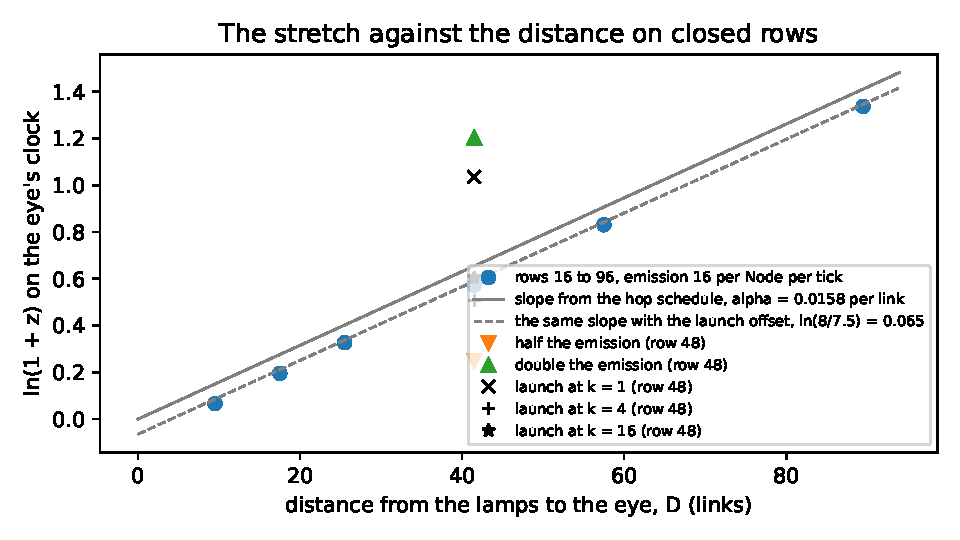
\includegraphics[width=0.85\linewidth]{figures/redshift_law.pdf}
\caption{$\ln(1+z)$ on the eye's clock against the distance for rows of 16 to 96 Nodes at one emission, with the slope read off the hop schedule; the runs at half and double the emission and at other launch hop times sit at $D = 41.5$.}
\end{figure}

\section{The hop time is a scale factor}\label{sec:scale}

Equations \eqref{eq:law} and \eqref{eq:distance} are the relations of a
Friedmann universe with $a(t) \propto k(t)$ and comoving distance $D$: light
emitted at $t_e$ and received at $t_o$ has $1 + z = a(t_o)/a(t_e)$ and
$D = \int dt / a$, and durations dilate by $1 + z$. The lattice is static and
nothing recedes, but for these two observables it cannot be told from
expansion with the matching history. Which history the load supplies decides
the low-redshift deceleration parameter: $k \propto t^n$ gives $q_0 = -(n-1)/n$,
so constant emission ($n = 1$) is the coasting universe and emission growing
with age ($n = 2$) accelerates with $q_0 = -1/2$, the value of flat
$\Lambda$CDM with $\Omega_m = 1/3$. The correspondence is exact: any
$a(t)$, $\Lambda$CDM included, is reproduced by $k(t) \propto a(t)$. Only
the linear history was run on the lattice; the others enter through
\eqref{eq:distance} as the continuum family of the same rule. This is a
kinematic correspondence and its limit at once: it covers the two
observables that depend only on $D(z)$ and on the stretch of durations, it
derives no dynamics (there is no Friedmann equation here and no equation of
state, only a load history put in by hand), and so the Hubble diagram and
the time dilation cannot decide between a growing load and an expanding
metric, while a lattice that fits them has explained nothing until it
derives its load history.

What a distant source looks like needs two more readings, both assumed
here rather than measured on the closed row. First, that the field of a
source dilutes as $1/D^2$ in three open dimensions: the row is one
dimensional and dilutes nothing; the $1/D^2$ is the isotropy probe of the
same simulator in open three-dimensional runs \cite{zenodo}, carried over.
Second, how a quantum's amount is read. Bodies arrive at a rate reduced by
$1 + z$ in every run. If each quantum keeps its amount (reading A) the
luminosity distance is $d_L = D\sqrt{1+z}$; if a quantum's energy is read
down by $1 + z$ as well (reading B) it is $d_L = D(1+z)$, the
expanding-universe form. The lattice measures that the frequency of a
phased ray falls by $1 + z$ under the default rule (the wave paragraph of
Section~\ref{sec:measure}); that a quantum's energy is its frequency, $E
\propto \nu$, is a relation the lattice does not contain, and reading B
rests on it as an assumption. The angular size of a source is $1/D$ in both
readings, so the surface brightness goes as $(1+z)^{-1}$ (A) or
$(1+z)^{-2}$ (B), against $(1+z)^{-4}$ for expansion.

\section{The supernova Hubble diagram}\label{sec:sn}

The Pantheon+ release \cite{scolnic2022,brout2022} lists 1701 type Ia
supernovae; we keep the 1580 Hubble-flow objects (not calibrators,
$z \ge 0.01$) with their corrected apparent magnitudes, and fit each shape
twice: with the diagonal errors, and with the full
statistical-plus-systematic covariance of the release restricted to the
kept objects. The diagonal fit is kept because the bins and residuals are
read from it; the covariance fit is the one whose $\Delta\chi^2$ is
quoted. Each shape $d(z)$ is fitted with one free offset (the absolute
magnitude and the scale $\alpha$ together, which are degenerate), so only
the shape of $m(z)$ is tested.

\begin{table}[H]\centering\footnotesize\setlength{\tabcolsep}{4pt}
\resizebox{\textwidth}{!}{%
\begin{tabular}{p{5.0cm}rrrrrp{5.6cm}}
\toprule
Shape & $q_0$ & $\chi^2_{\rm diag}$ & $\Delta\chi^2_{\rm diag}$ & $\chi^2_{\rm cov}$ & $\Delta\chi^2_{\rm cov}$ & model $-$ data by bin, mag\\
\midrule
Linear load, reading A & $1$ & 2511.8 & $+1817$ & 3278.5 & $+1891$ & $+0.22, 0.00, -0.22, -0.45, -0.93$\\
Linear load, reading B (coasting) & $0$ & 787.9 & $+93$ & 1492.8 & $+106$ & $+0.06, 0.00, -0.06, -0.07, -0.20$\\
Quadratic load, reading A & $1/2$ & 1356.7 & $+662$ & 2083.7 & $+697$ & $+0.14, 0.00, -0.14, -0.25, -0.55$\\
Quadratic load, reading B & $-1/2$ & 756.4 & $+62$ & 1450.8 & $+64$ & $-0.03, -0.00, +0.02, +0.12, +0.18$\\
Power law $k \propto t^{1.4}$, reading B (fitted $n$) & $-0.29$ & 699.3 & $+4.5$ & 1396.1 & $+9.0$ & $+0.01, -0.00, -0.01, +0.04, +0.01$\\
Best power law, reading A ($n = 5$) & $+0.20$ & 929.3 & $+234$ & 1639.3 & $+252$ & $+0.08, -0.00, -0.09, -0.13, -0.31$\\
Flat $\Lambda$CDM, $\Omega_m = 0.334$ & $-0.50$ & 694.8 & $0$ & 1387.1 & $0$ & $-0.01, +0.01, 0.00, +0.03, -0.10$\\
Einstein--de Sitter & $1/2$ & 1356.7 & $+662$ & 2083.7 & $+697$ & $+0.14, 0.00, -0.14, -0.25, -0.55$\\
\bottomrule
\end{tabular}}
\caption{Fits to the Pantheon+ Hubble-flow sample with one free offset each, with the diagonal errors (diag) and with the full statistical-plus-systematic covariance (cov); $q_0$ is the low-redshift deceleration parameter of the luminosity-distance shape, $1 - d''(0)/d'(0)$, which for reading A differs from that of the scale factor $k \propto t^n$ because the extra $\sqrt{1+z}$ enters the shape (for $n = 5$ the scale factor's $q_0$ is $-0.8$ and the shape's is $+0.20$). Bins $z = 0.01$--$0.1$, $0.1$--$0.3$, $0.3$--$0.6$, $0.6$--$1.0$, $1.0$--$2.3$ with 620, 466, 365, 104 and 25 objects, whose errors of the mean are 0.008, 0.009, 0.010, 0.024 and 0.062 mag, from the diagonal fit. Reading A and the quadratic load in reading A are the Einstein--de Sitter shape or worse; reading B with a fitted exponent is close to $\Lambda$CDM.}
\label{tab:sn}
\end{table}

Three things follow, and the full covariance changes none of them. The
reading in which only the arrival rate is redshifted (A) is excluded at
every exponent: its best power law is $\Delta\chi^2 = 252$ from
$\Lambda$CDM. The two load histories the model supplies by itself, constant
emission and emission growing with age, are disfavoured in reading B by
$\Delta\chi^2 = 106$ and $64$, with residuals that grow with redshift; the
quadratic history has the right $q_0$ and the wrong shape beyond $z \sim
0.5$. A power law with a fitted exponent, $n = 1.4$ ($q_0 = -0.29$), fits
within $\Delta\chi^2 = 9$ on 1580 objects, one parameter against
$\Lambda$CDM's one (the exponent is chosen on the diagonal fit and the
covariance $\chi^2$ evaluated at it). That is the correspondence of
Section~\ref{sec:scale} at work: the diagram can be fitted, and fitting it
says nothing until the exponent is derived.

\begin{figure}[H]\centering
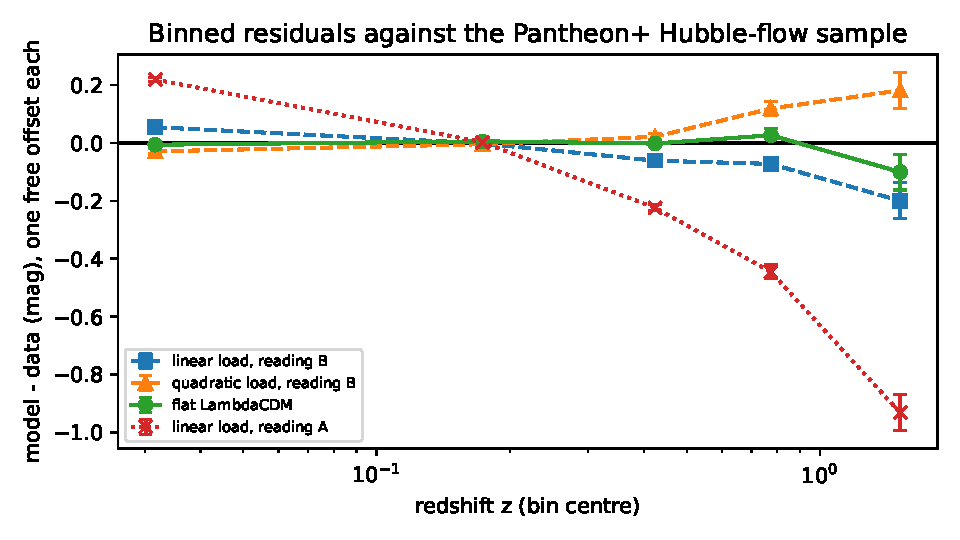
\includegraphics[width=0.85\linewidth]{figures/hubble_residuals.pdf}
\caption{Binned residuals, model minus data, of the shapes of Table~\ref{tab:sn} against the Pantheon+ sample; error bars are the errors of the bin means.}
\end{figure}

\section{The other two tests}\label{sec:tests}

\paragraph{Time dilation.} The law stretches durations by $1 + z$
(Table~\ref{tab:runs}, duration ratio, the same integers as $z$), because
every part of a signal waits the same hops. Supernova light curves dilate by $(1+z)^{1.07 \pm 0.06}$
\cite{blondin2008}; the lattice passes where tired light fails.

\paragraph{Surface brightness.} The Tolman test measures the exponent $n$ in
$\mathrm{SB} \propto (1+z)^{-n}$; expansion predicts $n = 4$, and Lubin and
Sandage \cite{lubin2001} find $n = 2.6$ to $3.4$ after correcting for
luminosity evolution, consistent with 4 and rejecting the tired-light $n = 1$.
The lattice predicts $n = 1$ in reading A and $n = 2$ in reading B, both
below the measured range: the lattice is in tension with this test now, not
awaiting it, and stays so unless the evolution correction absorbs a further
factor $(1+z)^{-1}$ or so, which is a claim about galaxies rather than about
the lattice. This is the test on which the lattice and expansion differ,
and we report it as unfavourable.

\paragraph{The temperature of the background.} $T(z) = T_0(1+z)$ tests a
blackbody spectrum's scaling; the lattice has no blackbody and the test
does not apply.

\section{What is not claimed}

\begin{itemize}
\item Not a derivation of the load history. The linear history is a
configured emission rule and the only one run on the lattice; an emission
growing with age couples the emitters' cycle count to the traffic through the
Node's single cycle and was not used; the history that fits the supernova
diagram ($n \approx 1.4$) is fitted, not derived, and the model has no rule
that produces it.
\item Not the removal of dark energy. The lattice relabels the acceleration
as a load growing faster than linearly; the unexplained quantity moves from
$\Lambda$ to the emission law and is not smaller for the move.
\item Not a passing of the Tolman test: the predicted exponent is below the
measured range in both readings.
\item Not a measured luminosity distance: the $1/D^2$ dilution is carried
over from open three-dimensional runs, and reading B takes a quantum's
energy to follow its measured frequency; the closed row measures rates,
durations and frequencies, not energies.
\item The wave sector is measured for a phased-ray train under both phase
rules, not for the causal source candidate's envelope, whose redshift is
not measured here.
\item Not a continuum result: every table is a finite row at a finite age;
the lattice quantizes the stretch in whole ticks, so $z$ resolves in steps of
$1/k_e$ per gap and every ``holds'' in this paper means within that
resolution; the load at a Node grows by the emission per tick (32 per tick
at $E = 32$, measured), so the hop schedule and $E/B$ agree.

\end{itemize}

What would make this a physics result: a rule of the lattice that fixes the
emission history, so that $n$ is derived rather than fitted; a measured
surface-brightness exponent that the same rule predicts; and the causal source candidate's envelope put through the same row.

\section*{Reproducibility}
The runs are produced by \texttt{redshift\_sweep.py} and the fits by
\texttt{redshift\_hubble.py} in the archived code \cite{zenodo}; the
supernova table is the public Pantheon+ release. Python 3.14; the lattice
runs use no floating point.

\begin{thebibliography}{99}
\bibitem{zwicky1929} F. Zwicky, Proc. Natl. Acad. Sci. 15, 773 (1929).
\bibitem{riess1998} A. G. Riess et al., Astron. J. 116, 1009 (1998).
\bibitem{perlmutter1999} S. Perlmutter et al., Astrophys. J. 517, 565 (1999).
\bibitem{scolnic2022} D. Scolnic et al., Astrophys. J. 938, 113 (2022).
\bibitem{brout2022} D. Brout et al., Astrophys. J. 938, 110 (2022).
\bibitem{blondin2008} S. Blondin et al., Astrophys. J. 682, 724 (2008).
\bibitem{lubin2001} L. M. Lubin and A. Sandage, Astron. J. 122, 1084 (2001).
\bibitem{paper1} A. Gonen, A finite-integer causal-lattice testbed: which resources reproduce interference, causal collapse and Bell correlations on one lattice (2026), arXiv preprint.
\bibitem{zenodo} A. Gonen, Universe24: a discrete simulator of local physical laws (Reality Theory), Zenodo (2026), doi:10.5281/zenodo.22738746.
\end{thebibliography}

\end{document}
